% !TEX program = xelatex
\documentclass[10pt, aspectratio=169]{beamer}
\usetheme{metropolis}
\metroset{sectionpage=none} % [핵심] 섹션 페이지(간지)를 생성하지 않음
\useoutertheme{metropolis}
\useinnertheme{metropolis}
\usecolortheme{metropolis}
\usefonttheme{professionalfonts} 

\usepackage{kotex}
\usepackage{pgfplots}
\pgfplotsset{compat=1.17}
\usepackage{graphicx, caption, hyperref, fontawesome5}
\usepackage{subcaption}
\usepackage{cleveref} % hyperref보다 나중에 불러와야 함
\usepackage{ulem} % 밑줄 긋기 (취소선 등)
\usepackage{lipsum} % 더미 텍스트 생성
\usepackage{fancybox, tcolorbox} % 박스 생성
\usepackage{tcolorbox}  % 박스 생성
\tcbuselibrary{skins, breakable, theorems}   % 박스 스킨 라이브러리
\usepackage{multicol}
% [수식 및 폰트 설정 - 기존 파일 그대로 유지]
\usepackage{amsmath}
\usepackage[math-style=ISO, bold-style=ISO]{unicode-math}
\usepackage{tikz}
\usetikzlibrary{positioning, shapes.geometric, arrows.meta, calc, fit, backgrounds, shapes.geometric, shadows.blur, shapes.symbols, decorations.pathmorphing, decorations.text}
\usefonttheme{professionalfonts}


%%%%%%%%%%%%%%%%%%%%%%%%%%%%%%%%%%%%%%%%%%%%%%%%%%%%
% 시스템 폰트가 아니라, ./fonts 폴더의 파일을 직접 사용합니다.
% 1. 영문/숫자 -> Fira Sans (Small Caps 지원)
\usepackage{fontspec}

% ---------------------------------------------------------
% [1] 영문/숫자 폰트 설정 (Fira Sans)
% ---------------------------------------------------------
% SmallCapsFont 옵션을 명시하지 않아도 OpenType 기능으로 자동 지원하지만,
% 확실하게 작동하도록 설정합니다.
\setmainfont{FiraSans-Regular.ttf}[
    Path = ../../fonts/,
    BoldFont = FiraSans-Bold.ttf,
    ItalicFont = FiraSans-Italic.ttf, % (있다면 추가, 없으면 생략 가능)
    AutoFakeSlant = 0.2
]

\setsansfont{FiraSans-Regular.ttf}[
    Path = ../../fonts/,
    BoldFont = FiraSans-Bold.ttf,
    ItalicFont = FiraSans-Italic.ttf,
    AutoFakeSlant = 0.2
]

% ---------------------------------------------------------
% [2] 한글 폰트 설정 (Noto Sans KR) - 한글에만 적용됨
% ---------------------------------------------------------
% \setmainhangulfont, \setsanshangulfont 명령은
% xetexko 패키지나 kotex 패키지를 사용할 때 유효합니다.
\setmainhangulfont{NotoSansKR-Regular.ttf}[
    Path = ../../fonts/,
    BoldFont = NotoSansKR-Bold.ttf,
    AutoFakeSlant = 0.2
]

\setsanshangulfont{NotoSansKR-Regular.ttf}[
    Path = ../../fonts/,
    BoldFont = NotoSansKR-Bold.ttf,
    AutoFakeSlant = 0.2
]

% 수식 폰트 설정
\setmathfont{Fira Math}
\setmathfont[range={up, bfup}, Scale=MatchLowercase, Path = ../../fonts/]{NotoSansKR-Regular.ttf}
\setmathfont[range={it, bfit}, Scale=MatchLowercase, FakeSlant=0.2, Path = ../../fonts/]{NotoSansKR-Regular.ttf}
% [Font Settings] Project-Local Fonts (Perfect Stability)

% [중요] 그림 경로 수정 (슬라이드 폴더 기준 2단계 위로)
% \graphicspath 명령은 중괄호 {} 안에 경로들을 나열하는 방식입니다.
% 마지막에 반드시 슬래시(/)를 붙여야 합니다.
\graphicspath{
    {./}                            % 1. 현재 tex 파일과 같은 폴더
    {../../assets/}                 % 2. 직접 만든 공용 벡터 이미지 (TikZ 결과물 등)
    {../../assets_extracted/ch02/}  % 3. (중요) 이 챕터의 자동 추출 이미지 폴더
}
%%%%%%%%%%%%%%%%%%%%%%%%%%%%%%%%%%%%%%%%%%%%%
% 이제 Fira Sans가 scshape를 지원하므로 정상 작동합니다.
% 1. 캡션 번호 활성화
\setbeamertemplate{caption}[numbered]
% 2. 캡션 폰트 크기 설정
\setbeamerfont{caption}{size=\scriptsize,shape=\itshape}
\setbeamerfont{section}{size=\footnotesize,shape=\scshape}
\setbeamerfont{subsection}{size=\scriptsize,shape=\itshape}
\setbeamerfont{section in toc}{shape=\scshape}

% 1. 제목 페이지(Title Page)의 메인 제목 설정
\setbeamerfont{subtitle}{shape=\itshape,size=\normalsize}
\setbeamerfont{title}{shape=\upshape,size=\Large}
% 2. 일반 슬라이드의 제목(Frame Title) 설정
\setbeamerfont{frametitle}{shape=\scshape, series=\mdseries}
% (선택사항) 섹션 페이지의 제목도 바꾸고 싶다면 아래 줄 추가
\setbeamerfont{section title}{shape=\scshape}
%%%%%%%%%%%%%%%%%%%%%%%%%%%%%%%%%%%%%%%%%%%%%%
%%%%%%%%%%%%%%%%%%%%%%%%%%%%%%%%%%%%%%%%%%%%%%
% 1. chapter라는 새로운 카운터 생성
\newcounter{chapter}
% 2. 챕터 번호 설정 (여기서 숫자를 바꾸면 됩니다)
\setcounter{chapter}{2}

% [Chapter Numbering] 현재 문서를 "Chapter 2"로 설정
% 섹션 번호 모양을 "2.1", "2.2" 형태로 강제 변경
\renewcommand{\thesection}{\thechapter.\arabic{section}}
% (선택사항) 서브섹션은 자동으로 "2.1.1"이 되지만, 확실하게 하려면 아래 줄도 추가
%\renewcommand{\thesubsection}{\thesection.\arabic{subsection}}
% Figure 2.x 형태로 출력 (chapter 번호 기준)
\renewcommand{\thefigure}{\thechapter.\arabic{figure}}
% Equation 2.x 형태로 출력 (chapter 번호 기준)
\renewcommand{\theequation}{\thechapter.\arabic{equation}}
\renewcommand{\figurename}{Fig.}

% --- [1] 본문 참조 설정 (\cref) ---
% \cref{label}을 썼을 때 "Fig. 번호"로 나오게 설정
% 형식: \crefname{타입}{단수형}{복수형}
\crefname{figure}{Fig.}{Figs.}
\Crefname{figure}{Fig.}{Figs.} % 문장 맨 앞 \Cref 용도

% --- [1] 번호 매기기 깊이 설정 ---
% 0: Chapter, 1: Section, 2: Subsection, 3: Subsubsection
% '1'로 설정하면 Section까지만 번호를 붙이고, Subsection부터는 번호를 생성하지 않습니다.
\setcounter{secnumdepth}{1} 

% --- [2] 목차(TOC) 스타일 설정 ---
% 2-1. 섹션: 번호 표시 (예: 1. Introduction)
\setbeamertemplate{section in toc}[sections numbered]
\setbeamertemplate{subsection in toc}{%
  \leavevmode
  \leftskip=1.0em
  {\color{gray}\textbullet} % 점을 회색으로 은은하게
  \hspace{0.5em}            % 적당한 간격
  {\footnotesize\inserttocsubsection}\par
}

% --- 매크로 정의 ---
% 사용법: \incfig{파일명(확장자제외)}{너비비율(0.0~1.0)}{캡션}
\newcommand{\incfig}[4]{%
    \begin{figure}
        \centering
        % 확장자를 생략하면 graphicspath에서 찾은 파일의 형식을 자동 인식합니다.
        \includegraphics[width=#2\textwidth]{#1} 
        \caption{#3}\label{#4}
    \end{figure}
}
% Preamble에 추가
\newcommand{\fakecaption}[2]{% #1: 참조할 라벨, #2: 텍스트
  \par\vspace{2pt}
  {\usebeamerfont{caption name}\usebeamercolor[fg]{caption name}\figurename~\ref{#1}:}%
  \hspace{1.0em}
  {\usebeamerfont{caption}\usebeamercolor[fg]{caption}\itshape #2}%
}

% 박스 매크로 정의
\newtcbox{\xmybox}[1][red]{on line,
arc=7pt,colback=#1!10!white,colframe=#1!50!black,
before upper={\rule[-3pt]{0pt}{10pt}},boxrule=1pt,
boxsep=0pt,left=6pt,right=6pt,top=2pt,bottom=2pt}

% --- [Colors] Starlink 전용 컬러 팔레트 정의 ---
\definecolor{space_bg}{HTML}{0B0E14}      % 배경: Deep Dark Navy
\definecolor{earth_top}{HTML}{1C2541}     % 지구 상단
\definecolor{earth_bot}{HTML}{000000}     % 지구 하단
\definecolor{starlink_cyan}{HTML}{00F0FF} % 레이저 링크 (Cyan Neon)
\definecolor{signal_green}{HTML}{00FF9D}  % LTE 신호 (Green Neon)
\definecolor{signal_orange}{HTML}{FF9E00} % Ku 신호 (Orange Neon)

% --- [Preamble] TikZ 스타일 전역 정의 (여기에 추가하세요) ---
\tikzset{
    % 빔 효과 (파라미터 #1을 여기서 안전하게 정의)
    beam_cone/.style={
        shade, 
        top color=#1, 
        bottom color=transparent!100, 
        shading angle=0, 
        opacity=0.7
    },
    % 레이저/선 효과
    glow_line/.style={
        line width=2pt, 
        color=#1, 
        opacity=0.8, 
        cap=round
    }
}
%%%%%%%%%%%%%%%%%%%%%%%%%%%%%%%%%%%%%%%%%%%%%%
%%%%%%%%%%%%%%%%%%%%%%%%%%%%%%%%%%%%%%%%%%%%%%

\subtitle{Communication Theory - 2026}
\title{Chapter 2. Signals and Signal Space}
\date{\today}
\author{
    이 경 근 \\
    {\tiny
        % \texorpdfstring{문서에 보일 내용}{PDF 속성에 들어갈 텍스트(특수문자 제외)}
        \texorpdfstring{\raisebox{-0.1ex}{\scalebox{0.85}{\faEnvelope}}}{} \href{mailto:infosec@knu.ac.kr}{infosec@knu.ac.kr} \quad 
        \texorpdfstring{\scalebox{0.9}{\faLinkedin}}{} \scalebox{0.9}{\href{https://www.linkedin.com/in/Kenny-0633-Lee}{Kenny-0633-Lee}}
    }
}
\institute{EE / KNU}

%%%%%%%%%%%%%%%%%%%%%%%%%%%%%%%%%%%%%%%%%%%%%%%
%%%%%%%%%%%%%%%%%%%%%%%%%%%%%%%%%%%%%%%%%%%%%%%
%%%%%%%%%%%%%%%%%%%%%%%%%%%%%%%%%%%%%%%%%%%%%%%

\begin{document}

% 1. 표지
\begin{frame}[plain]
    \titlepage
\end{frame}

% 2. 강의 목차
\begin{frame}{Table of Contents}
    \large
    \begin{multicols}{2} % 자동으로 2컬럼 배분
        \tableofcontents[hideallsubsections]
    \end{multicols}
\end{frame}

%%% Section 2 : Size of Signal %%%
\section{Size of A Signal}
\begin{frame}{Definition: Signal and System}
    \footnotesize{
    \tcbset{colback=red!5!white,fonttitle=\bfseries}    
    \begin{tcolorbox}[enhanced,title=\normalsize{Signal}, frame style={left color=red!75!black, right color=blue!75!black}]
        A signal is a set of information or data.\\
        The signals are functions of the independent variable \textbf{time $\mathbf{t}$}.
    \tcblower
    \begin{itemize}
        \item Examples: Audio signals, video signals, sensor data, etc.
    \end{itemize}
    \end{tcolorbox}

    \tcbset{colframe=red!5!black,fonttitle=\bfseries}
    \begin{tcolorbox}[enhanced,title=\normalsize{System}, frame style={left color=red!75!black, right color=blue!75!black}]
        Signals may be processed further by systems, which may modify them or extract additional infromation from them.\\
        Thus, a system is an entity that processes signals (\textbf{inputs}) to yield another set of signals (\textbf{outputs}).
    \tcblower
    \begin{itemize}
        \item For example, an antiaircraft radar system processes the received signals (inputs) to determine the position and velocity of an aircraft (outputs).
        \item More examples: Amplifiers, filters, modulators, demodulators, etc.
    \end{itemize}
    \end{tcolorbox}}
\end{frame}

% Energy vs Power Signals
\begin{frame}[c]
    \frametitle{Energy vs Power Signals}
    \begin{columns}
        % [왼쪽 컬럼] 그림 (a), (b) 배치 및 통합 캡션
        \begin{column}{0.45\textwidth}
            \begin{figure}
                \centering
                % (a) Energy Signal
                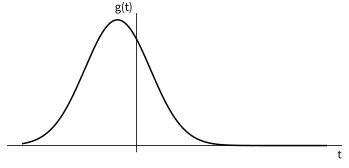
\includegraphics[width=0.8\textwidth]{fig_ch02_energy_sig} \\
                \vspace{-0.2cm} {\footnotesize (a) Signal with finite energy} \\
                \vspace{0.3cm} % (a)와 (b) 사이 간격
                
                % (b) Power Signal
                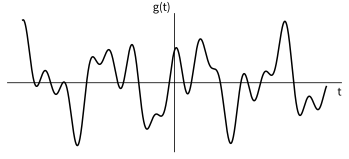
\includegraphics[width=0.8\textwidth]{fig_ch02_power_sig} \\
                \vspace{-0.2cm} {\footnotesize (b) Signal with finite power}
                
                % [통합 캡션] 맨 아래에 위치, 굵은 글씨 없음
                \caption{Examples of signals} \label{fig:2.1}
            \end{figure}
        \end{column}

        % [오른쪽 컬럼] 텍스트 설명
        \begin{column}{0.55\textwidth}
            {\footnotesize
            \begin{tcolorbox}[fonttitle=\sffamily\bfseries\small,title=Energy Signal]
                A signal is said to be an energy signal if its energy is finite and its average power approaches zero.
                \[
                E = \int_{-\infty}^{\infty} |g(t)|^2 dt < \infty, \quad P \rightarrow 0
                \]
            \end{tcolorbox}

            \vspace{0.2cm}
            
            \begin{tcolorbox}[fonttitle=\sffamily\bfseries\small,title=Power Signal]
                A signal is said to be a power signal if its average power is finite and its energy approaches infinite.
                \[
                P = \lim_{T \to \infty} \frac{1}{T} \int_{-T/2}^{T/2} |g(t)|^2 dt < \infty, \quad E \rightarrow \infty
                \]
            \end{tcolorbox}
            }
        \end{column}
    \end{columns} 
\end{frame}

% Units of Signal Energy and Power
\begin{frame}{Units of Signal Power}
    \begin{itemize}
        \item The standard units of signal energy and power are the "joule" and the "watt". 
        \item However, in practice, it is often customary to use logarithmic scales to describe signal power.
        \item A signal with average power of $P$ watts has power of either $P_{dBw}$ or $P_{dBm}$.
    \end{itemize}
    
    {\centering
    \begin{columns}
        \begin{column}{0.35\textwidth}
            \begin{tcolorbox}[colback=blue!5,before skip=6pt]
                $P_{dBw} = [10 \cdot \log_{10}P] \text{ dBw}$
            \end{tcolorbox}
        \end{column}
        \begin{column}{0.4\textwidth}
            \begin{tcolorbox}[colback=blue!5,before skip=6pt]
                $P_{dBm} = [30 + 10 \cdot \log_{10}P] \text{ dBm}$
            \end{tcolorbox}
        \end{column}
    \end{columns}
    }
    \begin{itemize}
        \item For example, \\
        \quad $P_{dBm} = -30 \text{ dBm} = 10^{-6} \text{W}$.
    \end{itemize}
\end{frame}

% Example 2.1
\begin{frame}[c]{Example 2.1}
\xmybox[blue]{\small\textbf{Q. Determine the suitable measures of the signals in \cref{fig:2.2}.}}
    \begin{columns}[c]
    % [왼쪽 컬럼] 그림 (a), (b)
    \begin{column}{0.3\textwidth}
        \begin{figure}[h]
            \centering
            \begin{tikzpicture}[scale=0.5, >=latex]
                \colorlet{signalcolor}{green!50!black}

                % --- (a) Graph ---
                \begin{scope}[shift={(0, 5.0)}]
                    % Axes
                    \draw[->] (-2.5, 0) -- (5.5, 0) node[below, scale=0.6] {$t$};
                    \draw[->] (0, -0.5) -- (0, 2.5) node[right, scale=0.6] {$g(t)$};
                    
                    % [수정] 원점 '0' (크기 절반)
                    \node[below right, scale=0.55] at (0,0) {0};

                    % [수정] Signal Waveform (진한 녹색)
                    % 1. t < 0 구간 (0, 수직선, 상수 구간)
                    \draw[thick, color=signalcolor] (-2.5, 0) -- (-1, 0) -- (-1, 2) -- (0, 2);
                    % 2. t >= 0 구간 (지수 함수)
                    \draw[thick, color=signalcolor, domain=0:5, samples=100] plot (\x, {2*exp(-\x/2)});
                    
                    % Label & Ticks
                    \node[scale=0.7] at (2.5, 1) {$2e^{-t/2}$};
                    
                    % [수정] x축 눈금 숫자 (크기 절반)
                    \draw (2, 0.1) -- (2, -0.1) node[below, scale=0.5] {2};
                    \draw (4, 0.1) -- (4, -0.1) node[below, scale=0.5] {4};
                    \draw (-1, 0.1) -- (-1, -0.1) node[below, scale=0.5] {-1};
                    
                    % [수정] y축 눈금 숫자 (크기 절반)
                    \node[scale=0.5] at (-0.2, 2) {2};
                    
                    \node[scale=0.7] at (4.5, 2) {(a)};
                \end{scope}

                % --- (b) Graph ---
                \begin{scope}[shift={(0, 1.0)}]
                    % Axes
                    \draw[->] (-4.5, 0) -- (4.8, 0) node[below, scale=0.6] {$t$};
                    \draw[->] (0, -1.5) -- (0, 1.5) node[right, scale=0.6] {$g(t)$};
                    
                    % [수정] 원점 '0' (크기 절반)
                    \node[below right, scale=0.55] at (0,0) {0};

                    % [수정] Sawtooth Wave Signal (진한 녹색)
                    \foreach \x in {-3, -1, 1, 3} {
                        \draw[thick, color=signalcolor] (\x, -1) -- (\x, 1); % 수직선
                    }
                    \foreach \x in {-5, -3, -1, 1, 3} {
                        \draw[thick, color=signalcolor] (\x, -1) -- (\x+2, 1); % 빗변
                    }
                    
                    % Dashed guide lines
                    \draw[dotted, thick] (0, 1) -- (1, 1);
                    \draw[dotted, thick] (0, -1) -- (-1, -1);
                    
                    % [수정] x축 눈금 숫자 (크기 절반)
                    \foreach \x in {-4, -3, -2, -1, 1, 2, 3, 4} {
                        \draw (\x, 0.1) -- (\x, -0.1) node[below, scale=0.5] {\x};
                    }
                    
                    % [수정] y축 눈금 숫자 (크기 절반)
                    \node[scale=0.5] at (0.3, 1) {1};
                    \node[scale=0.5] at (0.4, -1) {-1};
                    
                    \node[scale=0.7] at (4.5, 1.5) {(b)};
                \end{scope}
            \end{tikzpicture}
            \caption{Signal for Example} \label{fig:2.2}
        \end{figure}
    \end{column}

    \hfill

    %% [오른쪽 컬럼] 문제 및 풀이
    \begin{column}{0.6\textwidth}
        \scriptsize
        \begin{tcolorbox}[fonttitle=\bfseries,title=\cref{fig:2.2} (a)]
            Energy signal. Power approaches $0$ as $|t| \rightarrow \infty$.
            \[
                E_g = \int_{-\infty}^{\infty} |g(t)|^2 dt = \int_{-1}^{0}(2)^2 dt + \int_{0}^{\infty} 4e^{-t} dt = 4 + 4 = 8
            \]
        \end{tcolorbox}

        \vspace{0.05cm}

        \begin{tcolorbox}[fonttitle=\bfseries,title=\cref{fig:2.2} (b)]
            Power signal. Averaging $|g|^2(t)$ over an infinitely large interval is equivalent to averaging it over one period (2 seconds).
            \begin{eqnarray*}
            P_g  & = & \lim_{T \to \infty} \frac{1}{T} \int_{-T/2}^{T/2} |g(t)|^2 dt  = \frac{1}{T} \int_{-T/2}^{T/2} |g(t)|^2 dt \\
              & = & \frac{1}{2} \int_{-1}^{1} t^2 dt = \frac{1}{3}
            \end{eqnarray*}
        \end{tcolorbox}
    \end{column}

    \end{columns}
\end{frame}


% 2.2 Classification of signals
\section{Classification of Signals}
\begin{frame}{Classification of Signals}
    \begin{enumerate}
        \item Continuous time and discrete time signals
        \item Analog and digital signals
        \item Periodic and aperiodic signals
        \item Energy and power signals
        \item Deterministic and probabilistic signals
    \end{enumerate}
\end{frame}

% 2.2.1 Continuous time vs discrete time signals
\subsection{Continuous Time vs Discrete Time Signals}
\begin{frame}[fragile]
    \frametitle{Figure 2.3 Continuous vs Discrete Time Signals}
    \centering
    
    \begin{columns}[T] % [T]: 상단 정렬
    % [왼쪽 컬럼] 그림 (a), (b)
    \begin{column}{0.35\textwidth}
    \begin{figure}[T, font=\footnotesize]
        \begin{tikzpicture}[scale=0.5, font=\scriptsize, >=latex]
            
            % [수정 1] (a) 그래프 위치를 위로 조금 더 올림 (3.5 -> 4.0)
            % (b)가 커질 공간을 확보하기 위함입니다.
            \begin{scope}[shift={(0, 5.5)}]
                \draw[->] (-0.5, 0) -- (10.5, 0); 
                \draw[->] (0, -1.0) -- (0, 2.5) node[right] {$g(t)$};
                \node[below left] at (0,0) {0};
                \draw[thick] plot[domain=0:10, samples=150] (\x, {3 * exp(-0.4*\x) * sin(45*\x)});
                \node at (5, -1.2) {(a)};
            \end{scope}

            % [수정 2] (b) 그래프 수직 스케일 키우기
            % 기존 0.15 -> 0.22 (약 1.5배 확대)
            \begin{scope}[shift={(0, -0.5)}]
                % 편의를 위해 스케일 팩터를 변수(\ys)로 정의 (여기만 바꾸면 높이 조절 가능)
                \def\ys{0.22} 

                % --- 축 그리기 ---
                \draw (0, 0) -- (10.5, 0);
                % 축 길이도 스케일에 맞춰 늘어남 (-10~\ys ~ 12~\ys)
                \draw (0, -10*\ys) -- (0, 12*\ys); 

                % --- Y축 눈금 ---
                \foreach \y in {-10, -5, 0, 5, 10} {
                    % 좌표에 \ys 곱하기
                    \draw (0, \y*\ys) -- (-0.1, \y*\ys) node[left, scale=0.8] {\y};
                }
                \draw (0, 12*\ys) -- (-0.1, 12*\ys) node[left, scale=0.8] {12};
                \node[right] at (0, 12*\ys) {$g(t)$};

                % --- X축 눈금 (변동 없음) ---
                \foreach \x/\year in {0/1980, 1.2/1983, 2.4/1986, 3.6/1989, 4.8/1992, 6.0/1995, 7.2/1998, 8.4/2001, 9.6/2004} {
                    \draw (\x, 0) -- (\x, -0.1);
                    \node[rotate=90, anchor=east, font=\tiny] at (\x, -0.15) {\year};
                }

                % --- 데이터 막대 ---
                \pgfmathsetseed{42}
                \foreach \i in {0,1,...,100} {
                    \pgfmathsetmacro{\x}{0.1 * \i} 
                    
                    % (데이터 생성 로직 동일)
                    \pgfmathsetmacro{\val}{6 * rnd - 1} 
                    \ifnum \i < 12 \pgfmathsetmacro{\val}{\val - 5} \fi
                    \ifnum \i > 12 \ifnum \i < 36 \pgfmathsetmacro{\val}{\val + 3} \fi\fi 
                    \ifnum \i > 40 \ifnum \i < 48 \pgfmathsetmacro{\val}{\val - 3} \fi\fi 
                    \ifnum \i > 48 \ifnum \i < 84 \pgfmathsetmacro{\val}{\val + 2} \fi\fi 
                    \ifnum \i > 84 \ifnum \i < 90 \pgfmathsetmacro{\val}{\val - 3} \fi\fi 

                    % [핵심] 높이에 \ys(0.22) 적용
                    \ifdim \x cm < 10.2cm
                        \draw[thick] (\x, 0) -- (\x, \val*\ys);
                    \fi
                }

                \node[below, scale=0.7] at (5.25, -2.2) {Annualized U.S. GDP quarterly percentage growth};
                \node at (5, -3.2) {(b)};
            \end{scope}
        \end{tikzpicture}
    \caption{Continuous vs Discrete Time Signals} \label{fig:2.3}
    \end{figure}
    \end{column}

    \hfill

    % [오른쪽 컬럼] 설명
    \begin{column}{0.55\textwidth}
        \scriptsize
        %\tcbset{colframe=red!5!black,fonttitle=\bfseries\footnotesize,fontupper=\scriptsize,fontlower=\scriptsize}
        %\begin{tcolorbox}[enhanced,title=\cref{fig:2.3} (a), frame style={left color=red!75!black, right color=blue!75!black}]
        \begin{tcolorbox}[fonttitle=\sffamily\bfseries\footnotesize,title=\cref{fig:2.3} (a)]
            \textbf{Continous time signals} are specified for every value of time $t$. Many examples including:
        \begin{itemize}
            \item Audio recordings in analog media like LP, magnetic cassette, or reel-to-reel tapes.
            \item Signals received through AM/FM radio channel.
        \end{itemize}
        \end{tcolorbox}

        %\vspace{0.05cm}
        \begin{tcolorbox}[fonttitle=\sffamily\bfseries\footnotesize,title=\cref{fig:2.3} (b)]    
        %\begin{tcolorbox}[enhanced,title=\cref{fig:2.3} (b), frame style={left color=red!75!black, right color=blue!75!black}]
            \textbf{Discrete time signals} are specified only at discrete points of $t = nT$. Many examples including:
        \begin{itemize}
            \item The quarterly gross domestic product (GDP), stock market daily averages, and monthly sales of a corporation.
            \item Audio signals formatted by MP3, HE-AAC, FLAC, or ALAC.
        \end{itemize}
        \end{tcolorbox}
    \end{column}
\end{columns}
\end{frame}

% 2.2.2 Analog and Digital Signals
% Figure 2.4 Exam ples of signals: (a) analog andconti nuous time,(b) digita and continuous time,(c) analog and discrete time, (d) digital and discrete time
\subsection{Analog and Digital Signals}
\begin{frame}[fragile]
    \frametitle{Figure 2.4 Classification of Signals}
    \centering

\begin{figure}[h]
    \begin{tikzpicture}[scale=0.7, font=\scriptsize, >=latex]
        % [차분한 색상 정의]
        \colorlet{myblue}{blue!40!gray}   % Analog 신호용
        \colorlet{myred}{red!40!gray}    % Digital 신호용
        
        % 공통 스타일 설정
        \tikzset{
            axis/.style={->, thick},
            analog/.style={thick, myblue},
            digital/.style={thick, myred},
            guideline/.style={help lines, gray!30, dashed}
        }

        % (b)와 (d)에서 공통으로 사용할 계단형 데이터 정의 (x/y)
        % 이 좌표들은 (b)의 꺾임점이며, (d)는 이 선상의 값을 샘플링함
        \def\digitalwave{(0,0) -- (0.8,0) -- (0.8,1) -- (2.2,1) -- (2.2,-0.8) -- (3.8,-0.8) -- (3.8,0.5) -- (5,0.5)}

        % --- (a) Analog & Continuous Time ---
        \begin{scope}[shift={(0,4.5)}]
            \draw[axis] (-0.5,0) -- (5.5,0) node[below] {$t$};
            \draw[axis] (0,-1.2) -- (0,1.5) node[right] {$g(t)$};
            \draw[analog] plot[domain=0:5, samples=150] (\x, {sin(80*\x)});
            \node[below] at (2.5, -1.3) {(a) Analog, Continuous-time};
        \end{scope}

        % --- (b) Digital & Continuous Time ---
        \begin{scope}[shift={(8,4.5)}]
            \draw[axis] (-0.5,0) -- (5.5,0) node[below] {$t$};
            \draw[axis] (0,-1.2) -- (0,1.5) node[right] {$g(t)$};
            \draw[digital] \digitalwave;
            \node[below] at (2.5, -1.3) {(b) Digital, Continuous-time};
        \end{scope}

        % --- (c) Analog & Discrete Time ---
        \begin{scope}[shift={(0,0)}]
            \draw[axis] (-0.5,0) -- (5.5,0) node[below] {$n$};
            \draw[axis] (0,-1.2) -- (0,1.5) node[right] {$g[n]$};
            \foreach \x in {0, 0.25, ..., 5} {
                \pgfmathsetmacro{\val}{sin(80*\x)}
                \draw[analog] (\x, 0) -- (\x, \val);
                \fill[myblue] (\x, \val) circle (1.2pt);
            }
            \node[below] at (2.5, -1.3) {(c) Analog, Discrete-time};
        \end{scope}

        % --- (d) Digital & Discrete Time (Synchronized with b) ---
        \begin{scope}[shift={(8,0)}]
            \draw[axis] (-0.5,0) -- (5.5,0) node[below] {$n$};
            \draw[axis] (0,-1.2) -- (0,1.5) node[right] {$g[n]$};
            
            % 양자화 가이드라인
            % \foreach \y in {-1, -0.8, 0, 0.5, 1} {
            %     \draw[guideline] (-0.2, \y) -- (5.2, \y);
            % }

            % (b)의 파형과 동일한 레벨을 샘플링하여 그리기
            \foreach \x in {0, 0.25, ..., 5} {
                % (b)의 계단 구간에 맞춰 y값을 프로그래밍적으로 할당
                \pgfmathsetmacro{\qval}{
                    (\x < 0.7) ? 0 : (
                    (\x < 2.2) ? 1 : (
                    (\x < 3.7) ? -0.8 : 0.5))
                }
                \draw[digital] (\x, 0) -- (\x, \qval);
                \fill[myred] (\x, \qval) circle (1.2pt);
            }
            \node[below] at (2.5, -1.3) {(d) Digital, Discrete-time};
        \end{scope}
    \end{tikzpicture}
    \caption{Classification of signals based on amplitude and time domains} \label{fig:2.4}
\end{figure}
\end{frame}


% 2.2.3 Periodic and Aperiodic Signals
\subsection{Periodic and Aperiodic Signals}
\begin{frame}[fragile]
\frametitle{Periodic and Aperiodic Signals}
%\centering

\begin{columns}[t] % [b]: 하단 정렬
    \begin{column}{0.45\textwidth}
    \begin{figure}
        \centering
        % 확장자를 생략하면 graphicspath에서 찾은 파일의 형식을 자동 인식합니다.
        \includegraphics[width=1.15\textwidth, height=2.8cm]{fig_ch02_05} 
        \caption{Periodic signal of period $T_0$}\label{fig:2.5}
    \end{figure}
    \end{column}

    \hfill

    \begin{column}{0.5\textwidth}
        %\tcbset{colframe=red!5!black,fonttitle=\bfseries\small,fontupper=\footnotesize,fontlower=\footnotesize}
        %\begin{tcolorbox}[enhanced,title=\cref{fig:2.5}, frame style={left color=red!75!black, right color=blue!75!black}]
        \begin{tcolorbox}[fonttitle=\sffamily\bfseries\small,title=\cref{fig:2.5}]
        A signal $g(t)$ is \textbf{periodic} if there exists a positive constant $T_0$. The smallest value of $T_0$ in Eq. (\theequation) is the \textbf{period} of $g(t)$.
        
        \tcblower
        
         \addtocounter{equation}{4}
        \begin{equation}
                g(t) = g(t + T_0) \text{\quad for all t}
        \end{equation} \label{eq:2.5}
        \end{tcolorbox}
    \end{column}
\end{columns}
\end{frame}

% 2.2.4 Energy and Power Signals
\subsection{Energy and Power Signals}
\begin{frame}[fragile]
    \frametitle{Energy vs Power Signals}
    \begin{columns}
        % [왼쪽 컬럼] 그림 (a), (b) 배치 및 통합 캡션
            % [왼쪽 컬럼] 그림 (a), (b)
    \begin{column}{0.3\textwidth}
        \centering
        \begin{tikzpicture}[scale=0.5, >=latex]
                \colorlet{signalcolor}{green!50!black}

                % --- (a) Graph ---
                \begin{scope}[shift={(0, 5.0)}]
                    % Axes
                    \draw[->] (-2.5, 0) -- (5.5, 0) node[below, scale=0.6] {$t$};
                    \draw[->] (0, -0.5) -- (0, 2.5) node[right, scale=0.6] {$g(t)$};
                    
                    % [수정] 원점 '0' (크기 절반)
                    \node[below right, scale=0.55] at (0,0) {0};

                    % [수정] Signal Waveform (진한 녹색)
                    % 1. t < 0 구간 (0, 수직선, 상수 구간)
                    \draw[thick, color=signalcolor] (-2.5, 0) -- (-1, 0) -- (-1, 2) -- (0, 2);
                    % 2. t >= 0 구간 (지수 함수)
                    \draw[thick, color=signalcolor, domain=0:5, samples=100] plot (\x, {2*exp(-\x/2)});
                    
                    % Label & Ticks
                    \node[scale=0.7] at (2.5, 1) {$2e^{-t/2}$};
                    
                    % [수정] x축 눈금 숫자 (크기 절반)
                    \draw (2, 0.1) -- (2, -0.1) node[below, scale=0.5] {2};
                    \draw (4, 0.1) -- (4, -0.1) node[below, scale=0.5] {4};
                    \draw (-1, 0.1) -- (-1, -0.1) node[below, scale=0.5] {-1};
                    
                    % [수정] y축 눈금 숫자 (크기 절반)
                    \node[scale=0.5] at (-0.2, 2) {2};
                    
                    \node[scale=0.7] at (4.5, 2) {(a)};
                \end{scope}

                % --- (b) Graph ---
                \begin{scope}[shift={(0, 1.0)}]
                    % Axes
                    \draw[->] (-4.5, 0) -- (4.8, 0) node[below, scale=0.6] {$t$};
                    \draw[->] (0, -1.5) -- (0, 1.5) node[right, scale=0.6] {$g(t)$};
                    
                    % [수정] 원점 '0' (크기 절반)
                    \node[below right, scale=0.55] at (0,0) {0};

                    % [수정] Sawtooth Wave Signal (진한 녹색)
                    \foreach \x in {-3, -1, 1, 3} {
                        \draw[thick, color=signalcolor] (\x, -1) -- (\x, 1); % 수직선
                    }
                    \foreach \x in {-5, -3, -1, 1, 3} {
                        \draw[thick, color=signalcolor] (\x, -1) -- (\x+2, 1); % 빗변
                    }
                    
                    % Dashed guide lines
                    \draw[dotted, thick] (0, 1) -- (1, 1);
                    \draw[dotted, thick] (0, -1) -- (-1, -1);
                    
                    % [수정] x축 눈금 숫자 (크기 절반)
                    \foreach \x in {-4, -3, -2, -1, 1, 2, 3, 4} {
                        \draw (\x, 0.1) -- (\x, -0.1) node[below, scale=0.5] {\x};
                    }
                    
                    % [수정] y축 눈금 숫자 (크기 절반)
                    \node[scale=0.5] at (0.3, 1) {1};
                    \node[scale=0.5] at (0.4, -1) {-1};
                    
                    \node[scale=0.7] at (4.5, 1.5) {(b)};
                \end{scope}
        \end{tikzpicture}
            % [통합 캡션] 맨 아래에 위치, 굵은 글씨 없음
            % 캡션 대신 이걸 사용 -> 번호는 Figure 2.1로 고정됨!
            \fakecaption{fig:2.2}{Energy vs Power Signals (Recap)}
    \end{column}

    \hfill

        % [오른쪽 컬럼] 텍스트 설명
    \begin{column}{0.55\textwidth}
            \footnotesize
            %\tcbset{colframe=red!5!black,fonttitle=\bfseries\small,fontupper=\footnotesize,fontlower=\scriptsize}
            %\begin{tcolorbox}[enhanced,title=\cref{fig:2.1}(a) Energy Signal, frame style={left color=red!75!black, right color=blue!75!black}]
            \begin{tcolorbox}[fonttitle=\sffamily\bfseries\small,title=\cref{fig:2.2}(a) Energy Signal]
            A signal is said to be an energy signal if its energy is finite and its average power approaches zero.
                \begin{equation}
                \int_{-\infty}^{\infty} |g(t)|^2 dt < \infty
                \end{equation}\label{eq:2.6}
            \end{tcolorbox}

            \vspace{0.1cm}
            
            %\begin{tcolorbox}[enhanced,title=\cref{fig:2.1}(b) Power Signal, frame style={left color=red!75!black, right color=blue!75!black}]
            \begin{tcolorbox}[fonttitle=\sffamily\bfseries\small,title=\cref{fig:2.2}(b) Power Signal]
            A signal is said to be a power signal if its average power is finite and its energy approaches infinite.
                \begin{equation}
                0< \lim_{T \to \infty} \frac{1}{T} \int_{-T/2}^{T/2} |g(t)|^2 dt < \infty
                \end{equation}\label{eq:2.7}
            \end{tcolorbox}
    \end{column}
    \end{columns} 
\end{frame}

% 2.2.5 Deterministic and Random Signals
\subsection{Deterministic and Random Signals}
\begin{frame}
\frametitle{Deterministic and Random Signals}
\centering
\begin{columns}[T] %
    \begin{column}{0.45\textwidth}
    % \incfig{fig_ch02_27}{1.0}{ }{fig:2.27}
    \end{column}
    %
    \hfill
    %
    \begin{column}{0.5\textwidth}
    %\tcbset{colframe=red!5!black,fonttitle=\bfseries\footnotesize,fontupper=\scriptsize,fontlower=\scriptsize}
    %\begin{tcolorbox}[enhanced,title=Time scaling a signal, frame style={left color=red!75!black, right color=blue!75!black}]
    \begin{tcolorbox}[fonttitle=\sffamily\bfseries\footnotesize,title= .]
        \begin{itemize}
            \item .
            \item .
        \end{itemize}
        %\tcblower
        \begin{equation}
            g(t) = 
        \end{equation}
    \end{tcolorbox}
    \end{column}
\end{columns}
\end{frame}

% Figure 2.6 Time shifting a signal
\begin{frame}
\frametitle{Time shifting a signal}
\centering
\begin{columns}[T] % [b]: 하단 정렬
    \begin{column}{0.45\textwidth}
    \incfig{fig_ch02_06}{1.0}{Time shifting a signal}{fig:2.6}
    \end{column}
    %
    \hfill
    %
    \begin{column}{0.5\textwidth}
        %\tcbset{colframe=red!5!black,fonttitle=\bfseries\footnotesize,fontupper=\scriptsize,fontlower=\scriptsize}
        %\begin{tcolorbox}[enhanced,title=Time shifting a signal, frame style={left color=red!75!black, right color=blue!75!black}]
        \begin{tcolorbox}[fonttitle=\sffamily\bfseries\footnotesize,title=\cref{fig:2.6} Time shifting a signal]
            \begin{itemize}
                \item .
                \item .
            \end{itemize}
            %\tcblower
            \begin{equation}
                g(t) = 
            \end{equation}
        \end{tcolorbox}
    \end{column}
\end{columns}
\end{frame}


% Figure Figure 2.7 Time scaling a signal
\begin{frame}
\frametitle{Time scaling a signal}
\centering
\begin{columns}[T] % [b]: 하단 정렬
    \begin{column}{0.45\textwidth}
    \incfig{fig_ch02_07}{1.0}{Time scaling a signal}{fig:2.7}
    \end{column}
    %
    \hfill
    %
    \begin{column}{0.5\textwidth}
    %\tcbset{colframe=red!5!black,fonttitle=\bfseries\footnotesize,fontupper=\scriptsize,fontlower=\scriptsize}
    %\begin{tcolorbox}[enhanced,title=Time scaling a signal, frame style={left color=red!75!black, right color=blue!75!black}]
    \begin{tcolorbox}[fonttitle=\sffamily\bfseries\footnotesize,title=\cref{fig:2.7} Time scaling a signal]
        \begin{itemize}
            \item .
            \item .
        \end{itemize}
        %\tcblower
        \begin{equation}
            g(t) = 
        \end{equation}
    \end{tcolorbox}
    \end{column}
\end{columns}
\end{frame}


% Figure 2.8 Examples of time compression and time expansion of signals
\begin{frame}
\frametitle{Examples of time compression and time expansion of signals}
\centering
\begin{columns}[T] % [b]: 하단 정렬
    \begin{column}{0.45\textwidth}
    \incfig{fig_ch02_08}{1.0}{Examples of time compression and time expansion of signals}{fig:2.8}
    \end{column}
    %
    \hfill
    %
    \begin{column}{0.5\textwidth}
    %\tcbset{colframe=red!5!black,fonttitle=\bfseries\footnotesize,fontupper=\scriptsize,fontlower=\scriptsize}
    %\begin{tcolorbox}[enhanced,title=Time scaling a signal, frame style={left color=red!75!black, right color=blue!75!black}]
    \begin{tcolorbox}[fonttitle=\sffamily\bfseries\footnotesize,title=\cref{fig:2.8}]
        \begin{itemize}
            \item .
            \item .
        \end{itemize}
        %\tcblower
        \begin{equation}
            g(t) = 
        \end{equation}
    \end{tcolorbox}
    \end{column}
\end{columns}
\end{frame}


% Figure 2.9 Time inversion (reflection) of a signal
\begin{frame}
\frametitle{Time inversion (reflection) of a signal}
\centering
\begin{columns}[T] % [b]: 하단 정렬
    \begin{column}{0.45\textwidth}
    \incfig{fig_ch02_09}{1.0}{Time inversion (reflection) of a signal}{fig:2.9}
    \end{column}
    %
    \hfill
    %
    \begin{column}{0.5\textwidth}
    %\tcbset{colframe=red!5!black,fonttitle=\bfseries\footnotesize,fontupper=\scriptsize,fontlower=\scriptsize}
    %\begin{tcolorbox}[enhanced,title=Time scaling a signal, frame style={left color=red!75!black, right color=blue!75!black}]
    \begin{tcolorbox}[fonttitle=\sffamily\bfseries\footnotesize,title=\cref{fig:2.9}]
        \begin{itemize}
            \item .
            \item .
        \end{itemize}
        %\tcblower
        \begin{equation}
            g(t) = 
        \end{equation}
    \end{tcolorbox}
    \end{column}
\end{columns}
\end{frame}


% Figure 2.10 Example of time inversion
\begin{frame}
\frametitle{Example of time inversion}
\centering
\begin{columns}[T] % [b]: 하단 정렬
    \begin{column}{0.45\textwidth}
    \incfig{fig_ch02_10}{1.0}{Example of time inversion}{fig:2.10}
    \end{column}
    %
    \hfill
    %
    \begin{column}{0.5\textwidth}
    %\tcbset{colframe=red!5!black,fonttitle=\bfseries\footnotesize,fontupper=\scriptsize,fontlower=\scriptsize}
    %\begin{tcolorbox}[enhanced,title=Time scaling a signal, frame style={left color=red!75!black, right color=blue!75!black}]
    \begin{tcolorbox}[fonttitle=\sffamily\bfseries\footnotesize,title=\cref{fig:2.10}]
        \begin{itemize}
            \item .
            \item .
        \end{itemize}
        %\tcblower
        \begin{equation}
            g(t) = 
        \end{equation}
    \end{tcolorbox}
    \end{column}
\end{columns}
\end{frame}


% Figure 2.11 (a) Unit impulse and (b) its approximation
\section{Unit Impulse Signal}
\begin{frame}
\frametitle{(a) Unit impulse and (b) its approximation}
\centering
\begin{columns}[T] % [b]: 하단 정렬
    \begin{column}{0.45\textwidth}
    \incfig{fig_ch02_11}{1.0}{(a) Unit impulse and (b) its approximation}{fig:2.11}
    \end{column}
    %
    \hfill
    %
    \begin{column}{0.5\textwidth}
    %\tcbset{colframe=red!5!black,fonttitle=\bfseries\footnotesize,fontupper=\scriptsize,fontlower=\scriptsize}
    %\begin{tcolorbox}[enhanced,title=Time scaling a signal, frame style={left color=red!75!black, right color=blue!75!black}]
    \begin{tcolorbox}[fonttitle=\sffamily\bfseries\footnotesize,title=\cref{fig:2.11}]
        \begin{itemize}
            \item .
            \item .
        \end{itemize}
        %\tcblower
        \begin{equation}
            g(t) = 
        \end{equation}
    \end{tcolorbox}
    \end{column}
\end{columns}
\end{frame}


% Figure 2.12 (a) Unit step function u(t). (b) Causal exponential e−atu(t)
\begin{frame}
\frametitle{(a) Unit step function $u(t)$. (b) Causal exponential $e^{−at}u(t)$}
\centering
\begin{columns}[T]
    \begin{column}{0.45\textwidth}
    \incfig{fig_ch02_12}{1.0}{(a) Unit step function $u(t)$. (b) Causal exponential $e^{−at}u(t)$}{fig:2.12}
    \end{column}
    %
    \hfill
    %
    \begin{column}{0.5\textwidth}
    %\tcbset{colframe=red!5!black,fonttitle=\bfseries\footnotesize,fontupper=\scriptsize,fontlower=\scriptsize}
    %\begin{tcolorbox}[enhanced,title=Time scaling a signal, frame style={left color=red!75!black, right color=blue!75!black}]
    \begin{tcolorbox}[fonttitle=\sffamily\bfseries\footnotesize,title=\cref{fig:2.12}]
        \begin{itemize}
            \item .
            \item .
        \end{itemize}
        %\tcblower
        \begin{equation}
            g(t) = 
        \end{equation}
    \end{tcolorbox}
    \end{column}
\end{columns}
\end{frame}


% Section 2.4 Signals vs Vectors
\section{Signals versus Vectors}
\begin{frame}{Signals versus Vectors}
.
\end{frame}


% 2.4.1 Component of a Vector along Another Vector
% Figure 2.13 Component (projection) of a vector along another vector
\subsection{Component of a Vector along Another Vector}
\begin{frame}
\frametitle{Component (projection) of a vector along another vector}
\centering
\begin{columns}[T] %
    \begin{column}{0.45\textwidth}
    \incfig{fig_ch02_13}{1.0}{Component (projection) of a vector along another vector}{fig:2.13}
    \end{column}
    %
    \hfill
    %
    \begin{column}{0.5\textwidth}
    %\tcbset{colframe=red!5!black,fonttitle=\bfseries\footnotesize,fontupper=\scriptsize,fontlower=\scriptsize}
    %\begin{tcolorbox}[enhanced,title=Time scaling a signal, frame style={left color=red!75!black, right color=blue!75!black}]
    \begin{tcolorbox}[fonttitle=\sffamily\bfseries\footnotesize,title=\cref{fig:2.13}]
        \begin{itemize}
            \item .
            \item .
        \end{itemize}
        %\tcblower
        \begin{equation}
            g(t) = 
        \end{equation}
    \end{tcolorbox}
    \end{column}
\end{columns}
\end{frame}


% Figure 2.14 Approximations of a vector in terms of another vector
\begin{frame}
\frametitle{Approximations of a vector in terms of another vector}
\centering
\begin{columns}[T] %
    \begin{column}{0.45\textwidth}
    \incfig{fig_ch02_14}{1.0}{Approximations of a vector in terms of another vector}{fig:2.14}
    \end{column}
    %
    \hfill
    %
    \begin{column}{0.5\textwidth}
    %\tcbset{colframe=red!5!black,fonttitle=\bfseries\footnotesize,fontupper=\scriptsize,fontlower=\scriptsize}
    %\begin{tcolorbox}[enhanced,title=Time scaling a signal, frame style={left color=red!75!black, right color=blue!75!black}]
    \begin{tcolorbox}[fonttitle=\sffamily\bfseries\footnotesize,title=\cref{fig:2.14}]
        \begin{itemize}
            \item .
            \item .
        \end{itemize}
        %\tcblower
        \begin{equation}
            g(t) = 
        \end{equation}
    \end{tcolorbox}
    \end{column}
\end{columns}
\end{frame}


% 2.4.2 Decomposition of a Signal and Signal Components
\subsection{Decomposition of a Signal and Signal Components}
\begin{frame}{Decomposition of a Signal and Signal Components}
.
\end{frame}


% Example 2.2
% Figure 2.15 Approximation of square signal in terms of a single sinusoid
\begin{frame}
\frametitle{Approximation of square signal in terms of a single sinusoid}
\centering
\begin{columns}[T] %
    \begin{column}{0.45\textwidth}
    \incfig{fig_ch02_15}{1.0}{Approximation of square signal in terms of a single sinusoid}{fig:2.15}
    \end{column}
    %
    \hfill
    %
    \begin{column}{0.5\textwidth}
    %\tcbset{colframe=red!5!black,fonttitle=\bfseries\footnotesize,fontupper=\scriptsize,fontlower=\scriptsize}
    %\begin{tcolorbox}[enhanced,title=Time scaling a signal, frame style={left color=red!75!black, right color=blue!75!black}]
    \begin{tcolorbox}[fonttitle=\sffamily\bfseries\footnotesize,title=\cref{fig:2.15}]
        \begin{itemize}
            \item .
            \item .
        \end{itemize}
        %\tcblower
        \begin{equation}
            g(t) = 
        \end{equation}
    \end{tcolorbox}
    \end{column}
\end{columns}
\end{frame}


% 2.4.3 Complex Signal Space and Orthogonality
\subsection{Complex Signal Space and Orthogonality}
\begin{frame}{Complex Signal Space and Orthogonality}
. 
\end{frame}


% 2.4.4 Energy of the Sum of Orthogonal Signals
\subsection{Energy of the Sum of Orthogonal Signals}
\begin{frame}{Energy of the Sum of Orthogonal Signals}
.
\end{frame}


% Figure 2.16 Signals for Example 2.6
\begin{frame}
\frametitle{Signals for Example 2.6}
\centering
\begin{columns}[T] %
    \begin{column}{0.45\textwidth}
    \incfig{fig_ch02_16}{1.0}{Signals for Example 2.6}{fig:2.16}
    \end{column}
    %
    \hfill
    %
    \begin{column}{0.5\textwidth}
    %\tcbset{colframe=red!5!black,fonttitle=\bfseries\footnotesize,fontupper=\scriptsize,fontlower=\scriptsize}
    %\begin{tcolorbox}[enhanced,title=Time scaling a signal, frame style={left color=red!75!black, right color=blue!75!black}]
    \begin{tcolorbox}[fonttitle=\sffamily\bfseries\footnotesize,title=\cref{fig:2.16}]
        \begin{itemize}
            \item .
            \item .
        \end{itemize}
        %\tcblower
        \begin{equation}
            g(t) = 
        \end{equation}
    \end{tcolorbox}
    \end{column}
\end{columns}
\end{frame}


% Section 2.5 Correlation of signals
\section{Correlation of Signals}
\begin{frame}{Correlation of Signals}
. 
\end{frame}


% 2.5.1 Correlation Functions
\subsection{Correlation Functions}
\begin{frame}{Correlation Functions}
. 
\end{frame}


% 2.5.2 Autocorrelation Functions
% Figure 2.17 Physical explanation of the auto-correlation function
\subsection{Autocorrelation Functions}
\begin{frame}
\frametitle{Physical explanation of the auto-correlation function}
\centering
\begin{columns}[T] %
    \begin{column}{0.45\textwidth}
    \incfig{fig_ch02_17}{1.0}{Physical explanation of the auto-correlation function}{fig:2.17}
    \end{column}
    %
    \hfill
    %
    \begin{column}{0.5\textwidth}
    %\tcbset{colframe=red!5!black,fonttitle=\bfseries\footnotesize,fontupper=\scriptsize,fontlower=\scriptsize}
    %\begin{tcolorbox}[enhanced,title=Time scaling a signal, frame style={left color=red!75!black, right color=blue!75!black}]
    \begin{tcolorbox}[fonttitle=\sffamily\bfseries\footnotesize,title=\cref{fig:2.17}]
        \begin{itemize}
            \item .
            \item .
        \end{itemize}
        %\tcblower
        \begin{equation}
            g(t) = 
        \end{equation}
    \end{tcolorbox}
    \end{column}
\end{columns}
\end{frame}


% Figure 2.18 Representation of a vector in three-dimensional space
\begin{frame}
\frametitle{Representation of a vector in three-dimensional space}
\centering
\begin{columns}[T] %
    \begin{column}{0.45\textwidth}
    \incfig{fig_ch02_18}{1.0}{Representation of a vector in three-dimensional space}{fig:2.18}
    \end{column}
    %
    \hfill
    %
    \begin{column}{0.5\textwidth}
    %\tcbset{colframe=red!5!black,fonttitle=\bfseries\footnotesize,fontupper=\scriptsize,fontlower=\scriptsize}
    %\begin{tcolorbox}[enhanced,title=Time scaling a signal, frame style={left color=red!75!black, right color=blue!75!black}]
    \begin{tcolorbox}[fonttitle=\sffamily\bfseries\footnotesize,title=\cref{fig:2.18}]
        \begin{itemize}
            \item .
            \item .
        \end{itemize}
        %\tcblower
        \begin{equation}
            g(t) = 
        \end{equation}
    \end{tcolorbox}
    \end{column}
\end{columns}
\end{frame}


% Section 2.6 Orthogonal Signal Set
% 2.6.1 Orthogonal Vector Space
\section{Orthogonal Signal Set}
\subsection{Orthogonal Vector Space}
\begin{frame}{Orthogonal Vector Space}
. 
\end{frame}


% 2.6.2 Orthogonal Signal Space
\subsection{Orthogonal Signal Space}
\begin{frame}{Orthogonal Signal Space}
. 
\end{frame}


% 2.6.3 Parseval's Theorem
\subsection{Parseval's Theorem}
\begin{frame}{Parseval's Theorem}
. 
\end{frame}


% Section 2.7 The Exponential Fourier Series
\section{The Exponential Fourier Series}



% Figure 2.19
\begin{frame}
\frametitle{.}
\centering
\begin{columns}[T] %
    \begin{column}{0.45\textwidth}
    \incfig{fig_ch02_19}{1.0}{.}{fig:2.19}
    \end{column}
    %
    \hfill
    %
    \begin{column}{0.5\textwidth}
    %\tcbset{colframe=red!5!black,fonttitle=\bfseries\footnotesize,fontupper=\scriptsize,fontlower=\scriptsize}
    %\begin{tcolorbox}[enhanced,title=Time scaling a signal, frame style={left color=red!75!black, right color=blue!75!black}]
    \begin{tcolorbox}[fonttitle=\sffamily\bfseries\footnotesize,title=\cref{fig:2.19}]
        \begin{itemize}
            \item .
            \item .
        \end{itemize}
        %\tcblower
        \begin{equation}
            g(t) = 
        \end{equation}
    \end{tcolorbox}
    \end{column}
\end{columns}
\end{frame}


% Figure 2.20
\begin{frame}
\frametitle{ . }
\centering
\begin{columns}[T] %
    \begin{column}{0.45\textwidth}
    \incfig{fig_ch02_20}{1.0}{ . }{fig:2.20}
    \end{column}
    %
    \hfill
    %
    \begin{column}{0.5\textwidth}
    %\tcbset{colframe=red!5!black,fonttitle=\bfseries\footnotesize,fontupper=\scriptsize,fontlower=\scriptsize}
    %\begin{tcolorbox}[enhanced,title=Time scaling a signal, frame style={left color=red!75!black, right color=blue!75!black}]
    \begin{tcolorbox}[fonttitle=\sffamily\bfseries\footnotesize,title=\cref{fig:2.20}]
        \begin{itemize}
            \item .
            \item .
        \end{itemize}
        %\tcblower
        \begin{equation}
            g(t) = 
        \end{equation}
    \end{tcolorbox}
    \end{column}
\end{columns}
\end{frame}


% Figure 2.21
\begin{frame}
\frametitle{ . }
\centering
\begin{columns}[T] %
    \begin{column}{0.45\textwidth}
    \incfig{fig_ch02_21}{1.0}{ . }{fig:2.21}
    \end{column}
    %
    \hfill
    %
    \begin{column}{0.5\textwidth}
    %\tcbset{colframe=red!5!black,fonttitle=\bfseries\footnotesize,fontupper=\scriptsize,fontlower=\scriptsize}
    %\begin{tcolorbox}[enhanced,title=Time scaling a signal, frame style={left color=red!75!black, right color=blue!75!black}]
    \begin{tcolorbox}[fonttitle=\sffamily\bfseries\footnotesize,title=\cref{fig:2.21}]
        \begin{itemize}
            \item .
            \item .
        \end{itemize}
        %\tcblower
        \begin{equation}
            g(t) = 
        \end{equation}
    \end{tcolorbox}
    \end{column}
\end{columns}
\end{frame}


% Figure 2.22
\begin{frame}
\frametitle{ . }
\centering
\begin{columns}[T] %
    \begin{column}{0.45\textwidth}
    \incfig{fig_ch02_22}{1.0}{ . }{fig:2.22}
    \end{column}
    %
    \hfill
    %
    \begin{column}{0.5\textwidth}
    %\tcbset{colframe=red!5!black,fonttitle=\bfseries\footnotesize,fontupper=\scriptsize,fontlower=\scriptsize}
    %\begin{tcolorbox}[enhanced,title=Time scaling a signal, frame style={left color=red!75!black, right color=blue!75!black}]
    \begin{tcolorbox}[fonttitle=\sffamily\bfseries\footnotesize,title=\cref{fig:2.22}]
        \begin{itemize}
            \item .
            \item .
        \end{itemize}
        %\tcblower
        \begin{equation}
            g(t) = 
        \end{equation}
    \end{tcolorbox}
    \end{column}
\end{columns}
\end{frame}


% Figure 2.23
\begin{frame}
\frametitle{ . }
\centering
\begin{columns}[T] %
    \begin{column}{0.45\textwidth}
    \incfig{fig_ch02_23}{1.0}{ . }{fig:2.23}
    \end{column}
    %
    \hfill
    %
    \begin{column}{0.5\textwidth}
    %\tcbset{colframe=red!5!black,fonttitle=\bfseries\footnotesize,fontupper=\scriptsize,fontlower=\scriptsize}
    %\begin{tcolorbox}[enhanced,title=Time scaling a signal, frame style={left color=red!75!black, right color=blue!75!black}]
    \begin{tcolorbox}[fonttitle=\sffamily\bfseries\footnotesize,title=\cref{fig:2.23}]
        \begin{itemize}
            \item .
            \item .
        \end{itemize}
        %\tcblower
        \begin{equation}
            g(t) = 
        \end{equation}
    \end{tcolorbox}
    \end{column}
\end{columns}
\end{frame}


% Figure 2.24
\begin{frame}
\frametitle{.}
\centering
\begin{columns}[T] %
    \begin{column}{0.45\textwidth}
    \incfig{fig_ch02_24}{1.0}{ . }{fig:2.24}
    \end{column}
    %
    \hfill
    %
    \begin{column}{0.5\textwidth}
    %\tcbset{colframe=red!5!black,fonttitle=\bfseries\footnotesize,fontupper=\scriptsize,fontlower=\scriptsize}
    %\begin{tcolorbox}[enhanced,title=Time scaling a signal, frame style={left color=red!75!black, right color=blue!75!black}]
    \begin{tcolorbox}[fonttitle=\sffamily\bfseries\footnotesize,title=\cref{fig:2.24}]
        \begin{itemize}
            \item .
            \item .
        \end{itemize}
        %\tcblower
        \begin{equation}
            g(t) = 
        \end{equation}
    \end{tcolorbox}
    \end{column}
\end{columns}
\end{frame}


% Figure 2.25
\begin{frame}
\frametitle{ . }
\centering
\begin{columns}[T] %
    \begin{column}{0.45\textwidth}
    \incfig{fig_ch02_25}{1.0}{ . }{fig:2.25}
    \end{column}
    %
    \hfill
    %
    \begin{column}{0.5\textwidth}
    %\tcbset{colframe=red!5!black,fonttitle=\bfseries\footnotesize,fontupper=\scriptsize,fontlower=\scriptsize}
    %\begin{tcolorbox}[enhanced,title=Time scaling a signal, frame style={left color=red!75!black, right color=blue!75!black}]
    \begin{tcolorbox}[fonttitle=\sffamily\bfseries\footnotesize,title=\cref{fig:2.25}]
        \begin{itemize}
            \item .
            \item .
        \end{itemize}
        %\tcblower
        \begin{equation}
            g(t) = 
        \end{equation}
    \end{tcolorbox}
    \end{column}
\end{columns}
\end{frame}


% Figure 2.26
\begin{frame}
\frametitle{ . }
\centering
\begin{columns}[T] %
    \begin{column}{0.45\textwidth}
    \incfig{fig_ch02_26}{1.0}{ . }{fig:2.26}
    \end{column}
    %
    \hfill
    %
    \begin{column}{0.5\textwidth}
    %\tcbset{colframe=red!5!black,fonttitle=\bfseries\footnotesize,fontupper=\scriptsize,fontlower=\scriptsize}
    %\begin{tcolorbox}[enhanced,title=Time scaling a signal, frame style={left color=red!75!black, right color=blue!75!black}]
    \begin{tcolorbox}[fonttitle=\sffamily\bfseries\footnotesize,title=\cref{fig:2.26}]
        \begin{itemize}
            \item .
            \item .
        \end{itemize}
        %\tcblower
        \begin{equation}
            g(t) = 
        \end{equation}
    \end{tcolorbox}
    \end{column}
\end{columns}
\end{frame}


% Section 2.8 Matlab Exercise
\section*{Matlab Exercise}

% Figure 2.27
\begin{frame}
\frametitle{ . }
\centering
\begin{columns}[T] %
    \begin{column}{0.45\textwidth}
    \incfig{fig_ch02_27}{1.0}{ . }{fig:2.27}
    \end{column}
    %
    \hfill
    %
    \begin{column}{0.5\textwidth}
    %\tcbset{colframe=red!5!black,fonttitle=\bfseries\footnotesize,fontupper=\scriptsize,fontlower=\scriptsize}
    %\begin{tcolorbox}[enhanced,title=Time scaling a signal, frame style={left color=red!75!black, right color=blue!75!black}]
    \begin{tcolorbox}[fonttitle=\sffamily\bfseries\footnotesize,title=\cref{fig:2.27}]
        \begin{itemize}
            \item .
            \item .
        \end{itemize}
        %\tcblower
        \begin{equation}
            g(t) = 
        \end{equation}
    \end{tcolorbox}
    \end{column}
\end{columns}
\end{frame}


% Figure 2.28
\begin{frame}
\frametitle{ . }
\centering
\begin{columns}[T] %
    \begin{column}{0.45\textwidth}
    \incfig{fig_ch02_28}{1.0}{ }{fig:2.28}
    \end{column}
    %
    \hfill
    %
    \begin{column}{0.5\textwidth}
    %\tcbset{colframe=red!5!black,fonttitle=\bfseries\footnotesize,fontupper=\scriptsize,fontlower=\scriptsize}
    %\begin{tcolorbox}[enhanced,title=Time scaling a signal, frame style={left color=red!75!black, right color=blue!75!black}]
    \begin{tcolorbox}[fonttitle=\sffamily\bfseries\footnotesize,title=\cref{fig:2.28}]
        \begin{itemize}
            \item .
            \item .
        \end{itemize}
        %\tcblower
        \begin{equation}
            g(t) = 
        \end{equation}
    \end{tcolorbox}
    \end{column}
\end{columns}
\end{frame}


% Figure 2.29
\begin{frame}
\frametitle{ . }
\centering
\begin{columns}[T] %
    \begin{column}{0.45\textwidth}
    \incfig{fig_ch02_29}{1.0}{ . }{fig:2.29}
    \end{column}
    %
    \hfill
    %
    \begin{column}{0.5\textwidth}
    %\tcbset{colframe=red!5!black,fonttitle=\bfseries\footnotesize,fontupper=\scriptsize,fontlower=\scriptsize}
    %\begin{tcolorbox}[enhanced,title=Time scaling a signal, frame style={left color=red!75!black, right color=blue!75!black}]
    \begin{tcolorbox}[fonttitle=\sffamily\bfseries\footnotesize,title=\cref{fig:2.29}]
        \begin{itemize}
            \item .
            \item .
        \end{itemize}
        %\tcblower
        \begin{equation}
            g(t) = 
        \end{equation}
    \end{tcolorbox}
    \end{column}
\end{columns}
\end{frame}


% Figure 2.30
\begin{frame}
\frametitle{ . }
\centering
\begin{columns}[T] %
    \begin{column}{0.45\textwidth}
    \incfig{fig_ch02_30}{1.0}{ . }{fig:2.30}
    \end{column}
    %
    \hfill
    %
    \begin{column}{0.5\textwidth}
    %\tcbset{colframe=red!5!black,fonttitle=\bfseries\footnotesize,fontupper=\scriptsize,fontlower=\scriptsize}
    %\begin{tcolorbox}[enhanced,title=Time scaling a signal, frame style={left color=red!75!black, right color=blue!75!black}]
    \begin{tcolorbox}[fonttitle=\sffamily\bfseries\footnotesize,title=\cref{fig:2.30}]
        \begin{itemize}
            \item .
            \item .
        \end{itemize}
        %\tcblower
        \begin{equation}
            g(t) = 
        \end{equation}
    \end{tcolorbox}
    \end{column}
\end{columns}
\end{frame}


% Figure 2.31
\begin{frame}
\frametitle{ . }
\centering
\begin{columns}[T] %
    \begin{column}{0.45\textwidth}
    \incfig{fig_ch02_31}{1.0}{ . }{fig:2.31}
    \end{column}
    %
    \hfill
    %
    \begin{column}{0.5\textwidth}
    %\tcbset{colframe=red!5!black,fonttitle=\bfseries\footnotesize,fontupper=\scriptsize,fontlower=\scriptsize}
    %\begin{tcolorbox}[enhanced,title=Time scaling a signal, frame style={left color=red!75!black, right color=blue!75!black}]
    \begin{tcolorbox}[fonttitle=\sffamily\bfseries\footnotesize,title=\cref{fig:2.31}]
        \begin{itemize}
            \item .
            \item .
        \end{itemize}
        %\tcblower
        \begin{equation}
            g(t) = 
        \end{equation}
    \end{tcolorbox}
    \end{column}
\end{columns}
\end{frame}


% Figure 2.32
\begin{frame}
\frametitle{ . }
\centering
\begin{columns}[T] %
    \begin{column}{0.45\textwidth}
    \incfig{fig_ch02_32}{1.0}{ . }{fig:2.32}
    \end{column}
    %
    \hfill
    %
    \begin{column}{0.5\textwidth}
    %\tcbset{colframe=red!5!black,fonttitle=\bfseries\footnotesize,fontupper=\scriptsize,fontlower=\scriptsize}
    %\begin{tcolorbox}[enhanced,title=Time scaling a signal, frame style={left color=red!75!black, right color=blue!75!black}]
    \begin{tcolorbox}[fonttitle=\sffamily\bfseries\footnotesize,title=\cref{fig:2.32}]
        \begin{itemize}
            \item .
            \item .
        \end{itemize}
        %\tcblower
        \begin{equation}
            g(t) = 
        \end{equation}
    \end{tcolorbox}
    \end{column}
\end{columns}
\end{frame}


% Figure 2.33
\begin{frame}
\frametitle{ . }
\centering
\begin{columns}[T] %
    \begin{column}{0.45\textwidth}
    \incfig{fig_ch02_33}{1.0}{ . }{fig:2.33}
    \end{column}
    %
    \hfill
    %
    \begin{column}{0.5\textwidth}
    %\tcbset{colframe=red!5!black,fonttitle=\bfseries\footnotesize,fontupper=\scriptsize,fontlower=\scriptsize}
    %\begin{tcolorbox}[enhanced,title=Time scaling a signal, frame style={left color=red!75!black, right color=blue!75!black}]
    \begin{tcolorbox}[fonttitle=\sffamily\bfseries\footnotesize,title=\cref{fig:2.33}]
        \begin{itemize}
            \item .
            \item .
        \end{itemize}
        %\tcblower
        \begin{equation}
            g(t) = 
        \end{equation}
    \end{tcolorbox}
    \end{column}
\end{columns}
\end{frame}


% Figure 2.34
\begin{frame}
\frametitle{ . }
\centering
\begin{columns}[T] %
    \begin{column}{0.45\textwidth}
    \incfig{fig_ch02_34}{1.0}{ . }{fig:2.34}
    \end{column}
    %
    \hfill
    %
    \begin{column}{0.5\textwidth}
    %\tcbset{colframe=red!5!black,fonttitle=\bfseries\footnotesize,fontupper=\scriptsize,fontlower=\scriptsize}
    %\begin{tcolorbox}[enhanced,title=Time scaling a signal, frame style={left color=red!75!black, right color=blue!75!black}]
    \begin{tcolorbox}[fonttitle=\sffamily\bfseries\footnotesize,title=\cref{fig:2.34}]
        \begin{itemize}
            \item .
            \item .
        \end{itemize}
        %\tcblower
        \begin{equation}
            g(t) = 
        \end{equation}
    \end{tcolorbox}
    \end{column}
\end{columns}
\end{frame}

% Problems
\section*{Problems}


% Figure 2.35
\begin{frame}
\frametitle{ . }
\centering
\begin{columns}[T] %
    \begin{column}{0.45\textwidth}
    \incfig{fig_ch02_35}{1.0}{ . }{fig:2.35}
    \end{column}
    %
    \hfill
    %
    \begin{column}{0.5\textwidth}
    %\tcbset{colframe=red!5!black,fonttitle=\bfseries\footnotesize,fontupper=\scriptsize,fontlower=\scriptsize}
    %\begin{tcolorbox}[enhanced,title=Time scaling a signal, frame style={left color=red!75!black, right color=blue!75!black}]
    \begin{tcolorbox}[fonttitle=\sffamily\bfseries\footnotesize,title=\cref{fig:2.35}]
        \begin{itemize}
            \item .
            \item .
        \end{itemize}
        %\tcblower
        \begin{equation}
            g(t) = 
        \end{equation}
    \end{tcolorbox}
    \end{column}
\end{columns}
\end{frame}


% Summary
\section*{Summary}
\begin{frame}
\frametitle{Summary}

\end{frame}
\end{document}